\documentclass[conference]{IEEEtran}
\IEEEoverridecommandlockouts
% The preceding line is only needed to identify funding in the first footnote. If that is unneeded, please comment it out.
\usepackage{cite}
\usepackage{amsmath,amssymb,amsfonts}
\usepackage{algorithmic}
\usepackage{graphicx}
\usepackage{textcomp}
\usepackage{xcolor}
\def\BibTeX{{\rm B\kern-.05em{\sc i\kern-.025em b}\kern-.08em
    T\kern-.1667em\lower.7ex\hbox{E}\kern-.125emX}}
\begin{document}

\title{Medical Abstract Segmentation Using Natural Language Processing\\}

\author{\IEEEauthorblockN{Saifuddin Shaikh}
\IEEEauthorblockA{
\textit{SCTR's Pune Institute of Computer Technology}
Pune, India \\
Department of Information Technology\\
saifuddinshaikh818@gmail.com}
\and
\IEEEauthorblockN{Pranish Warke}
\IEEEauthorblockA{
\textit{SCTR's Pune Institute of Computer Technology}
Pune, India \\
Department of Information Technology\\
pranish2402@gmail.com}
\and
\IEEEauthorblockN{Dr. Emmanuel M.}
\IEEEauthorblockA{
\textit{ SCTR's Pune Institute of Computer Technology}
Pune, India \\
Department of Information Technology\\
emmanuelm@pict.edu}
\and
\IEEEauthorblockN{Rishikesh Suryavanshi}
\IEEEauthorblockA{
\textit{SCTR's Pune Institute of Computer Technology}
Pune, India \\
Department of Information Technology\\
rishits321@gmail.com}
}
\maketitle

\begin{abstract}
Randomized control trials (RCTs) are essential for
evaluating the effectiveness of medical interventions, but their
results are often buried within lengthy and complex documents.
Efficiently extracting and organizing critical information from
RCT abstracts can significantly impact evidence-based decision making
and healthcare research. The automated segmentation
of medical abstracts is a vital component of medical information
retrieval and analysis, significantly impacting clinical decision making,
healthcare research, and knowledge discovery. This
paper presents an innovative approach to segmenting abstracts
of RCTs through the application of natural language processing
(NLP) and neural networks. The practical applications of NLP
and neural network-based text segmentation in the context of
RCTs are exemplified, ranging from systematic reviews and meta analyses
to the development of clinical guidelines. Case studies are
presented to showcase the impact of this technology in improving
the accessibility and utilization of RCT results. This paper serves
as a valuable resource for researchers, healthcare professionals,
and data scientists, offering a glimpse into the future of RCT
abstract segmentation. It underscores the pivotal role of NLP
and neural networks in unlocking the potential of RCT data,
ultimately advancing the field of evidence-based medicine and
healthcare decision-making.

\end{abstract}
\begin{IEEEkeywords}
medical abstract,text segmentation,randomized
control trial (RCT),natural language processing(NLP),neural networks.
\end{IEEEkeywords} 

\section{Introduction}
A particular kind of study design that is frequently used in medical research to assess the efficacy of a treatment or intervention is the randomized controlled trial (RCT). An RCT compares the results of individuals who get the treatment or intervention with those of those who do not by randomly assigning participants to various groups. Current artificial neural network (ANN) based sentence categorization models frequently classify sentences on their own without taking the context into account.

Medical abstract segmentation for randomized controlled trials (RCTs) utilizing natural language processing (NLP) and neural networks has several applications that improve clinical decision-making, healthcare, and medical research. The growing amount of medical literature and the need for more effective methods to glean important insights from this enormous body of knowledge are driving the ongoing evolution of this profession.

Structured Randomized Controlled Trials (RCTs) are useful for a range of Natural Language Processing (NLP) tasks, including text summarization, information extraction, and retrieval. Sentences can be categorized into categories such as Background, Objective, Methods, Results, and Conclusion. Nonetheless, a significant portion of PubMed abstracts are not organized hierarchically. According to Ripple et al. (2014), only roughly 30\% of all PubMed abstracts contain their structural information, which makes it more difficult to effectively identify new information and retrieve information from those substantial biomedical bibliographic databases. Medical abstract sentence classification has been the focus of numerous research investigations.

Focusing on identifying sentences in medical abstracts especially those from randomized controlled trials (RCTs), which are often regarded as the greatest sources of medical evidence is the goal of "Medical Abstract Segmentation."

\section{Literature Survey}
A comprehensive study has been done on text classification
in the domain of medical research papers. Some of the most
recent and prominent ones have been used for this literature
survey.
In [1] the dataset consists of approximately 200,000 abstracts
of randomized controlled trials, totaling 2.3 million
sentences. Each sentence of each abstract is labeled with its
role in the abstract using one of the following classes: background,
objective, method, result, or conclusion, and PubMed
200k RCT is a substantial dataset designed for sequential
sentence classification, is introduced. It notably stands as
one of the largest datasets of its kind known to date. The
evaluation encompasses the performance assessment of various
baseline models, providing a valuable reference for researchers
to readily benchmark their algorithms without the necessity of
creating their own foundational benchmarks.
[2] suggests a novel uniform deep learning architecture
and multi-task learning approach for cross-domain sequential
sentence classification in scientific texts. This paper introduces
a comprehensive deep-learning architecture designed for
sequential sentence classification, demonstrating remarkable
advancements, particularly in full paper datasets, without the
need for intricate feature engineering. The authors conduct
a thorough investigation and comparison of transfer learning
approaches, shedding light on the exceptional effectiveness
of multi-task models applied across diverse datasets. Furthermore,
this study places significant emphasis on the crucial
notion of semantic relatedness between classes within varying
dataset annotation schemes. It proposes a practical and robust
method for identifying and establishing these semantic connections.
Such an approach bears the promise of unlocking
the potential for cross-discipline applications in the domain of
sentence classification, with particular relevance to academic
search engines and information retrieval systems.
Similarly [3] Adopted a deep learning neural network model
and pretrained the network on PubMed non-RCT dataset.
Transfer Learning with fine-tuning was done on the handlabeled
dataset they created from scratch. The PubMed-non-
RCT corpus was converted into a three-class dataset, and
their model was trained on it. They achieved 92.1% accuracy
on the PubMed-non-RCT dataset. The model was then
evaluated on various CS corpora using different approaches:
’Locally-trained,’ ’Pre-trained on PubMed,’ and ’Fine-tuned’.
Notably, ’Fine-tuned’ transfer learning significantly improved
the model, while ’Pre-trained on PubMed’ performed worse
than local training, indicating the dissimilarity between the
CS and biomedical corpora. Despite such differences, transfer
learning with fine-tuning still provided more than a 10%
accuracy boost, even with entirely dissimilar datasets. The
paper introduces a method for automatic discourse classification
in computer science abstracts, showing that transfer
learning with fine-tuning yields impressive results, even with
limited labeled data. The model effectively generalizes across
CS sub-fields, despite variations in discourse classification due
to presentation style differences.
In [4] The model is composed of four components: the word
embedding layer, the sentence encoding layer, the context
enriching layer, and the label sequence optimization layer.
The sequence of embedding vectors is first processed by a
bi-directional RNN (bi-RNN) or CNN layer. In this work,
they introduced an ANN-based hierarchical sequential labeling
network designed to classify sequentially appearing sentences
in text. By incorporating contextual information from neighboring
sentences through an LSTM layer, they observed a
significant enhancement in prediction quality. Their model
demonstrated a notable 2%-3% improvement over state-ofthe-
art results in two datasets focusing on sequential sentence
classification within medical abstracts. This proposed model’s
potential for generalization to various problems related to
sequential sentence classification, including paragraph-level
sequential sentence categorization in full-text articles, presents
promising opportunities for text mining and document retrieval.
In [5] The model consists of two novel components: supervised
local attention and an auxiliary span-based classification
task. The proposed model aims to capture the latent segment
structure of the document by considering the coherent semantics
of contiguous sentences. It utilizes dynamic local attention
to explicitly capture the structural information.
In [6] a Machine Learning approach that aims to classify
sentences according to the PIBOSO scheme is presented.
A discriminative set of features that do not rely on any
external resources to achieve results is used. In this paper,
they introduced a machine-learning approach for identifying
scientific artifacts in biomedical abstracts within the context
of Evidence-Based Medicine. Their approach utilized
sentence classification following the PIBOSO scheme. Importantly,
their approach did not rely on external resources
for classification features. The results demonstrated a significant
improvement over existing methods, achieving a microaverage
F-score of 90.74% and 87.21% for structured and
unstructured abstracts, respectively. This marks a substantial
increase compared to prior approaches.
In [7] visits clustering algorithm is implemented based on
the following four steps: Medical concepts are extracted from
free-text descriptions of an interview and examination, a new
representation of identified concepts is derived using concept
embedding, concept embeddings are transformed into visit
embeddings and clustering is performed on visit embeddings.
They used two of the most common: k-means and hierarchical
clustering with Ward’s method for merging clusters. These
algorithms cover two different clustering approaches. The
algorithms are memory and time-efficient, so no need to use
more advanced methods.
[8] and [9] propose a few-shot prompt learning-based approach
to classify sentences in medical abstracts of randomized
clinical trials (RCT) and observational studies (OS) to
subsections of Introduction, Background, Methods, Results,
and Conclusion. 5 manually designed templates in a combination
of 4 BERT model variants were tested and compared
to a previous Hierarchical Sequential Labeling Network architecture
and traditional BERT-based sentence classification
method. Four deep learning models, namely RNN, LSTM,
GRU, and BLSTM are used. Data pre-processing steps are
applied that include: text cleaning, tokenization, stemming,
as well as lemmatization to remove and stop words. Their
approach achieves state-of-the-art results on all three datasets,
surpassing Jin and Szolovits (2018) and their BERT-based
baselines. The performance gap between their baselines and
their best model is more pronounced for smaller datasets
(CSABSTRUCT, NICTA) and narrower for the larger dataset
(PUBMED-RCT), underlining the significance of pretraining
for smaller datasets. To delve into the advantages of their joint
sentence encoding relative to the BERT+Transformer baseline,
they qualitatively analyze examples from CSABSTRUCT.
They discover that a significant portion of such examples
require contextual information for accurate classification, emphasizing
the need for context in certain instances.

\begin{table*}%[h]
\begin{tabular}{|p{4.6cm}|p{6cm}|p{4.9cm}|p{1.95cm}|}
\hline
Title &
  Methodologies &
  Inferences &
  Dataset \\ \hline
\begin{tabular}[c]{@{}l@{}}PubMed 200k RCT: a Dataset for \\ Sequential Sentence \\ Classification in Medical Abstracts\end{tabular} &
  \begin{tabular}[c]{@{}l@{}}Dataset is constructed upon MED-\\ LINE/PubMed Baseline Database. \\ Abstracts are selected based on the\\ two criteria: \\ i. It must be an RCT\\ ii. It must be structured\end{tabular} &
  \begin{tabular}[c]{@{}l@{}}• It is the largest such dataset \\    in the field of Medical \\    Research.\\ • It evaluated the performance on \\   several baseline models \\   based on this dataset.\\ • It achieved state of the art results \\   for Bi-ANN model with \\   F1 score of 91.6\end{tabular} &
  \begin{tabular}[c]{@{}l@{}}PubMed \\ 200k RCT\end{tabular} \\ \hline
\begin{tabular}[c]{@{}l@{}}Cross-Domain Multi-Task \\ Learning for Sequential Sentence \\ Classification in Research Papers\end{tabular} &
  \begin{tabular}[c]{@{}l@{}}1. Proposed SciBERT-HSLN architecture.\\ 2. Utilized SciBERT for Word Embeddings.\\ 3. Two approaches are suggested here one \\ without Transfer Learning and one with \\     Transfer Learning.\end{tabular} &
  \begin{tabular}[c]{@{}l@{}}• It achieved state of the art results for \\    PMD dataset with F1 score of 93.1\\ • F1 score of 86.8 for NIC dataset\end{tabular} &
  \begin{tabular}[c]{@{}l@{}}PMD, NIC, \\ ART, DRI\end{tabular} \\ \hline
\begin{tabular}[c]{@{}l@{}}Segmenting Scientific Abstracts \\ into Discourse Categories: \\ A Deep Learning-Based Approach \\ for Sparse Labeled Data\end{tabular} &
  \begin{tabular}[c]{@{}l@{}} Transfer Learning with Fine Tuning was \\ done on the hand labelled dataset \\ they created from scratch.\end{tabular} &
  \begin{tabular}[c]{@{}l@{}}• It was able to achieve 75\% accuracy \\    with the classification of CS abstracts.\end{tabular} &
  \begin{tabular}[c]{@{}l@{}}Hand Labelled \\ corpus of \\ structured \\ CS abstracts\end{tabular} \\ \hline
\begin{tabular}[c]{@{}l@{}}Hierarchical Neural Networks \\ for Sequential Sentence \\ Classification in Medical \\ Scientific Abstracts\end{tabular} &
  \begin{tabular}[c]{@{}l@{}} Model is composed of four layers :\\     i.   Word Embedding layer\\     ii.  Sentence Encoding layer\\     iii. Context Enriching layer\\     iv.  Label Sequence Optimisation layer\end{tabular} &
  • F1 score for PubMed 20k dataset is 92.6 &
  PubMed 20k RCT \\ \hline
\begin{tabular}[c]{@{}l@{}}A Span-based Dynamic\\  Local Attention Model for \\ Sequential Sentence \\ Classification\end{tabular} &
  \begin{tabular}[c]{@{}l@{}} Model consists of two novel components:\\       i. supervised local attention\\       ii. auxiliary span based classification\end{tabular} &
  \begin{tabular}[c]{@{}l@{}}• F1 score of 92.8 on PubMed 20k RCT \\ • F1 score of 86.8 on NICTA-PIBOSO\end{tabular} &
  PubMed 20k RCT \\ \hline
\begin{tabular}[c]{@{}l@{}}Identifying scientific artefacts \\ in biomedical literature: \\ the Evidence Based Medicine \\ use case\end{tabular} &
  \begin{tabular}[c]{@{}l@{}}A machine learning approach that aims \\     to classify sentences according to\\     PIBOSO scheme is presented.\end{tabular} &
  \begin{tabular}[c]{@{}l@{}}• CRF classifier achieves F1 score of 90.74 \\    and 87.21 respectively over structured \\    and unstructured abstracts.\end{tabular} &
  NICTA-PIBOSO \\ \hline
\begin{tabular}[c]{@{}l@{}}Towards More Generalizable and \\ Accurate Sentence \\ Classification in \\ Medical Abstracts with Less Data\end{tabular} &
  \begin{tabular}[c]{@{}l@{}} Few shot prompt based learning approach to \\     classify\\     sentences in medical abstracts was discussed.\end{tabular} &
  \begin{tabular}[c]{@{}l@{}}• The study showed that the HSLN model \\    required only 20\% of the training data to \\    achieve comparable F1 scores when \\    compared with the baseline model.\end{tabular} &
  \begin{tabular}[c]{@{}l@{}}PubMed 200k/20k\\ PubMed 20k OS\end{tabular} \\ \hline
\begin{tabular}[c]{@{}l@{}}Interpretable segmentation \\ of medical free-text records \\ based on word\end{tabular} &
  \begin{tabular}[c]{@{}l@{}} K-Means and Hierarchical Clustering with \\ Ward's method was used.\end{tabular} &
  \begin{tabular}[c]{@{}l@{}}• The embeddings outperformed \\    Pennington \\    et al on medical term analogies despite a \\    smaller corpus size.\\ • Future work should explore the dynamic \\    relationship with identified clusters.\end{tabular} &
  \begin{tabular}[c]{@{}l@{}}The Polish corpus \\ of free text \\ clinical records\end{tabular} \\ \hline
\begin{tabular}[c]{@{}l@{}}Pretrained Language Models\\  for Sequential Sentence\\ Classification\end{tabular} &
  \begin{tabular}[c]{@{}l@{}} Four Deep Learning Models namely RNN, LSTM,\\     GRU and BLSTM are used.\end{tabular} &
  \begin{tabular}[c]{@{}l@{}}• Accuracy: BLSTM gives the highest \\    accuracy of 82.18\%\end{tabular} &
  \begin{tabular}[c]{@{}l@{}}Kaggle Dataset \\ having insult \\ labelled \\ comments \\ was used.\end{tabular} \\ \hline
\begin{tabular}[c]{@{}l@{}}Deep Learning Based Text Classification: \\ A Comprehensive Review\end{tabular} &
  \begin{tabular}[c]{@{}l@{}} Survey of more than 150 DL models was carried, \\     which are developed in the past six years \\     and have significantly improved \\     state of the art on various TC tasks\end{tabular} &
  \begin{tabular}[c]{@{}l@{}}• Several state of the art models were used\\    in this paper\end{tabular} &
  \begin{tabular}[c]{@{}l@{}}SQuAD,\\ WikiQA,\\ DBpedia\end{tabular} \\ \hline
\begin{tabular}[c]{@{}l@{}}Universal Language Model Fine-\\ tuning for Text Classification.\end{tabular} &
  \begin{tabular}[c]{@{}l@{}}\\  Proposed discriminative fine-tuning, slanted \\     triangular learning rates, and gradual unfreezing\end{tabular} &
  \begin{tabular}[c]{@{}l@{}}• Method suggested significantly \\    outperforms \\    the state-of-the-art  on six text \\    classification tasks, reducing the error  \\    by 18-24\% on the majority \\    of datasets.\end{tabular} &
  \begin{tabular}[c]{@{}l@{}}TREC-6\\ IMDb\\ Yelp-bi Yelp-full\\ DBpedia\\ AG\end{tabular} \\ \hline
\begin{tabular}[c]{@{}l@{}}A Hierarchical Model with Recurrent \\ Convolutional \\ Neural Networks for \\ Sequential Sentence Classification\end{tabular} &
  \begin{tabular}[c]{@{}l@{}} A new approach called SR-RCNN to generate \\     sentence encoding which uses both Bi-RNN \\     and text CNN to capture contextual and literal \\     relevance information\end{tabular} &
  \begin{tabular}[c]{@{}l@{}}• The model performs best on all datasets, \\    promoting previous best published \\    results by 0.5\%, 0.5\%and 2.5\% \\    on the PubMed 20k, PubMed 200k \\    and NICTA-PIBOSO dataset\end{tabular} &
  \begin{tabular}[c]{@{}l@{}}PubMed RCT,\\ NICTA-PIBOSO\end{tabular} \\ \hline
\begin{tabular}[c]{@{}l@{}}Sectioning of Biomedical Abstracts: \\ A Sequence of Sequence\\ Classification Task.\end{tabular} &
  \begin{tabular}[c]{@{}l@{}}1. It uses BIOBERT based model, with a moving\\     window to contextualise the abstracts.\\ 2. Proposed SSN-4 Model which has four layers:\\          i. word embedding layer\\          ii. sentence representation layer\\          iii. BLSTM layer\\          iv. CRF layer\end{tabular} &
  \begin{tabular}[c]{@{}l@{}}• The model trained with the MDS \\    performs fairly well in \\    both MDS and RCT data sets\end{tabular} &
  \begin{tabular}[c]{@{}l@{}}A new data set \\ called MDS \\ that is \\ considerably \\ bigger than \\ PubMed RCT\end{tabular} \\ \hline
\end{tabular}
\end{table*}

\newpage
\section{Proposed Methodology}
\begin{figure}[h]
  \centering
  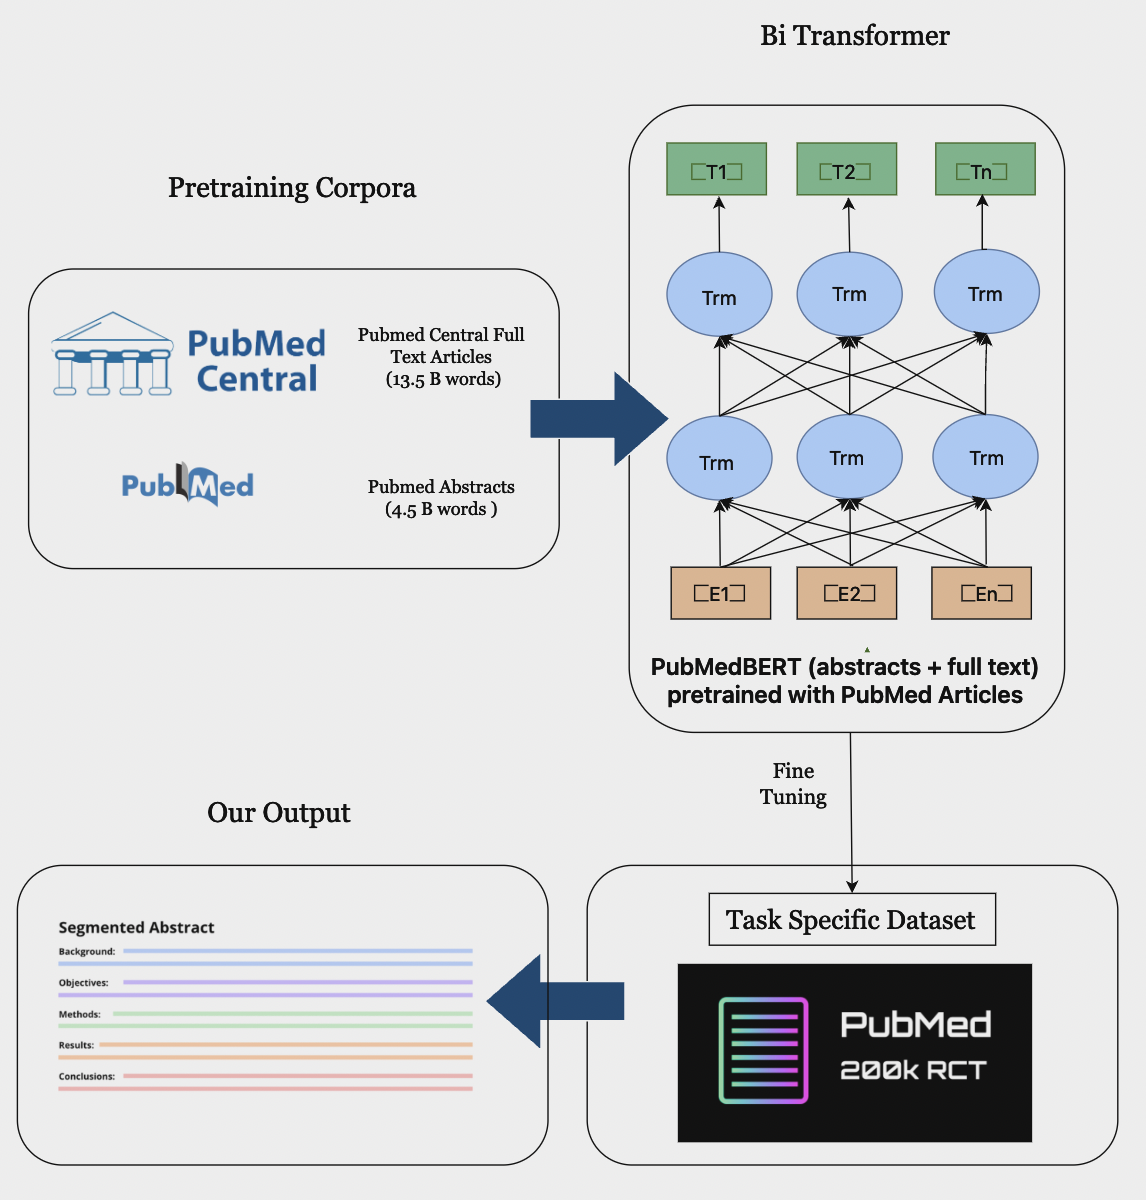
\includegraphics[width=8cm,height=10cm]{pubmed_architecture.png}
  \caption{Model Architechture}
  \label{fig:architectural}
\end{figure}
The model first takes abstract text as input. Data from 3 different datasets (Training Data, Validation Data and Test Data) is loaded.The data is distributed into 5 labels, namely Objectives,Methods,Conclusions,Background and Results.
\begin{figure}[h]
    \centering
    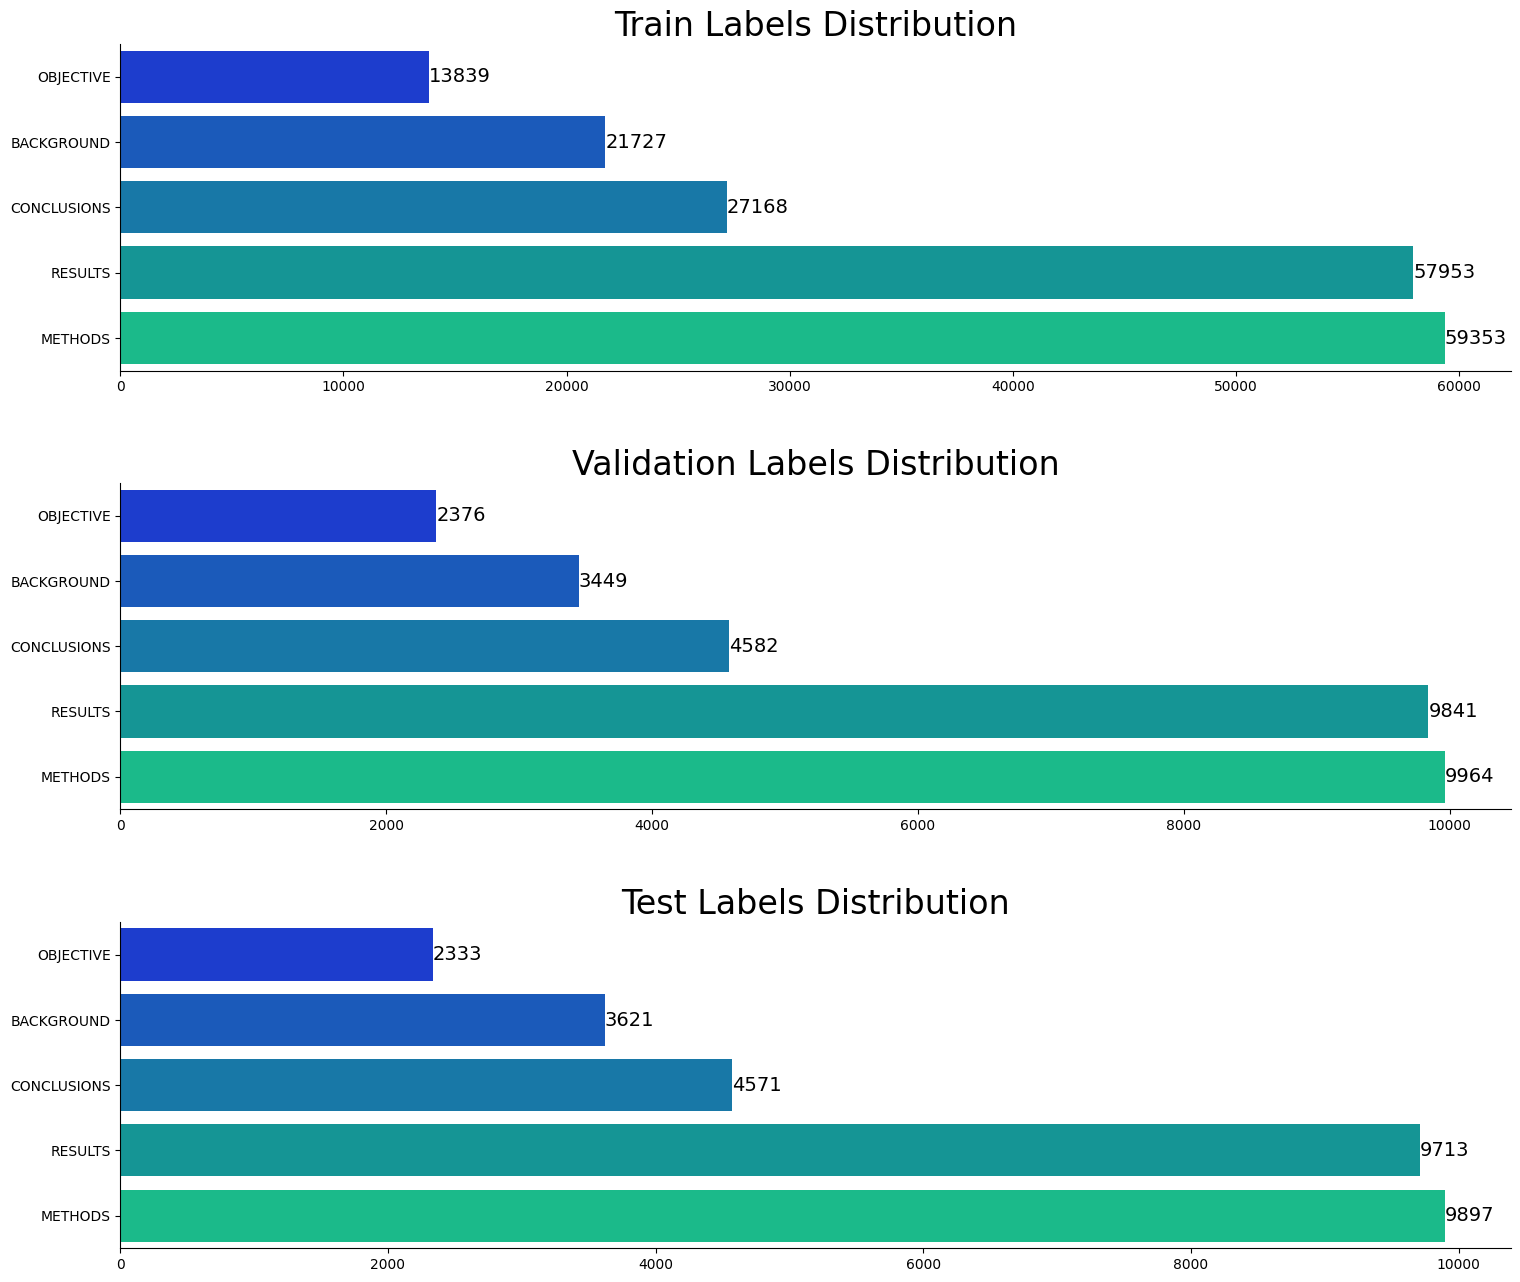
\includegraphics[width=9cm]{labels_distribution.png}
    \caption{Distribution of Labels}
    \label{fig: sequence diagram}
\end{figure}

For generating text segments using BERT model, we first apply tokenizer, inspect token count and the acquired tokens are then vector representation encoded, and the PubMedBERT model's fine tuning layer comes next. The key phases of the process are:
\begin{enumerate}
    \item \textbf{Data Exploration and Tokenization}
    \item \textbf{Transfer Learning Model: PubMedBERT}
    \item \textbf{Train Model}
    \item \textbf{Performance Analysis}
    \item \textbf{Predict on Actual Real Abstract}
\end{enumerate}


\subsection{Dataset Sources}

This study made use of the PubMed 20K RCT dataset. https://github.com/Franck-Dernoncourt/pubmed-rct is where you may access the dataset. There are 2.3 million terms in the collection drawn from around 200,000 abstracts of randomized controlled trials. Every sentence in an abstract is given a class according to its function inside the abstract, such as background, objective, method, result, or conclusion.

For the specified problem of medical abstract segmentation,
PubMed dataset is publicly available. It consists of following
five labels and the number of samples are as follows:

\begin{enumerate}
    \item METHODS 59353
    \item RESULTS 57953
    \item CONCLUSIONS 27168
    \item BACKGROUND 21727
    \item OBJECTIVE 13839
\end{enumerate}

\subsection{Data Exploration and Tokenization}

In this process,firstly we have inspected the distribution of labels in Training data,validation data and test data. Plotting a bar graph for all 3 datasets gives a fair idea about label distribution. We used the AutoTokenizer  class from the transformers library to dynamically load a tokenizer for a specific pre-trained model which is microsoft/BiomedNLP-PubMedBERT-base-uncased-abstract-fulltext. For applications like natural language processing and comprehension, where text inputs must be transformed into numerical representations that can be analyzed by machine learning models, tokenization is crucial.

\subsection{Transfer Learning Model: PubMedBERT}
A version of the BERT (Bidirectional Encoder Representations from Transformers) model created especially for biomedical text is called PubMedBERT. It makes use of the concepts of transfer learning, which is the process of optimizing a model that has been pre-trained on a sizable corpus of text for a subsequent task. PubMedBERT leveraged two new techniques—Enhanced Mask Decoder and Disentangled Attention Mechanism—to improve upon the BERT (Bidirectional Encoder Representations from Transformers) and RoBERTa models. Each word is characterized by the Disentangled Attention Mechanism using two different vectors to encode its position and content, respectively. This makes it possible for the model to more accurately represent the connections between words and where they belong in a sentence. During model pre-training, the Improved Mask Decoder takes the place of the SoftMax layer to predict masked tokens.



\subsection{Train Model}
The model we are using is fine tuned using the pre-trained microsoft/BiomedNLP-PubMedBERT-base-uncased-abstract-fulltext model. We must set up an input pipeline to load, preprocess, and feed the tokenized texts to the model in order for it to be trained. This pipeline is necessary because tokenizing every text at once could result in an out of memory error. In order to expedite the training process and allocate GPU memory efficiently, we also employ a large batch size.

Since this is a text segmentation problem, we will use cross-entropy as the loss function to train the model. We will employ the Adam optimizer with 0.001 as the (default) learning rate in terms of the optimizer. We will only monitor the accuracy and loss metrics while the model is being trained.

During training, the learning rate is dynamically adjusted using the ReduceLROnPlateau scheduler. The ReduceLROnPlateau scheduler helps stabilize the optimization process by reducing the learning rate when the model's performance on a validation set stops improving. Also, the ReduceLROnPlateau scheduler helps prevent over fitting by adjusting the learning rate based on the model's performance on a validation set. 


\section{Experimentation Results and Empirical Analysis}

The problems with the relevant samples are indicated by the F1-Score for OBJECTIVE and BACKGROUND. The model's performance, however, is comparable to the earlier deep learning models like RoBERTa, BERT and BioBERT.
\begin{figure}[h]
    \centering
    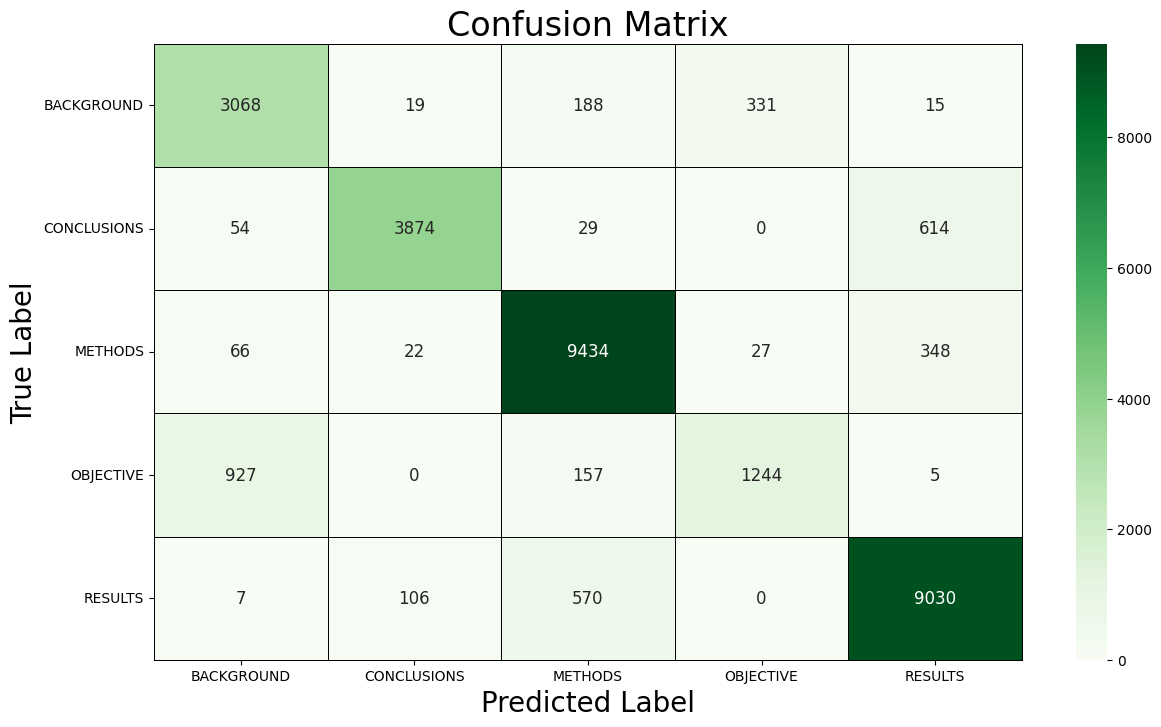
\includegraphics[width=9cm]{confusion_matrix.png}
    \caption{Confusion Matrix}
    \label{fig: sequence diagram}
\end{figure}

\begin{table}[h]
\centering
\caption{Classification Metrics}
\label{tab:classification_metrics}
\begin{tabular}{|l|ccc|c|}
\hline
\multirow{\textbf{Class}} & \multicolumn{3}{c}{\textbf{Metrics}} & \multirow{\textbf{Support}} \\ \cline{1-5}
 & \textbf{Precision} & \textbf{Recall} & \textbf{F1-score} &  \\ \hline
BACKGROUND & 0.74 & 0.85 & 0.79 & 3621 \\
CONCLUSIONS & 0.96 & 0.85 & 0.90 & 4571 \\
METHODS & 0.91 & 0.95 & 0.93 & 9897 \\
OBJECTIVE & 0.78 & 0.53 & 0.63 & 2333 \\
RESULTS & 0.90 & 0.93 & 0.92 & 9713 \\ \hline
\end{tabular}
\end{table}

\begin{figure}[h]
    \centering
    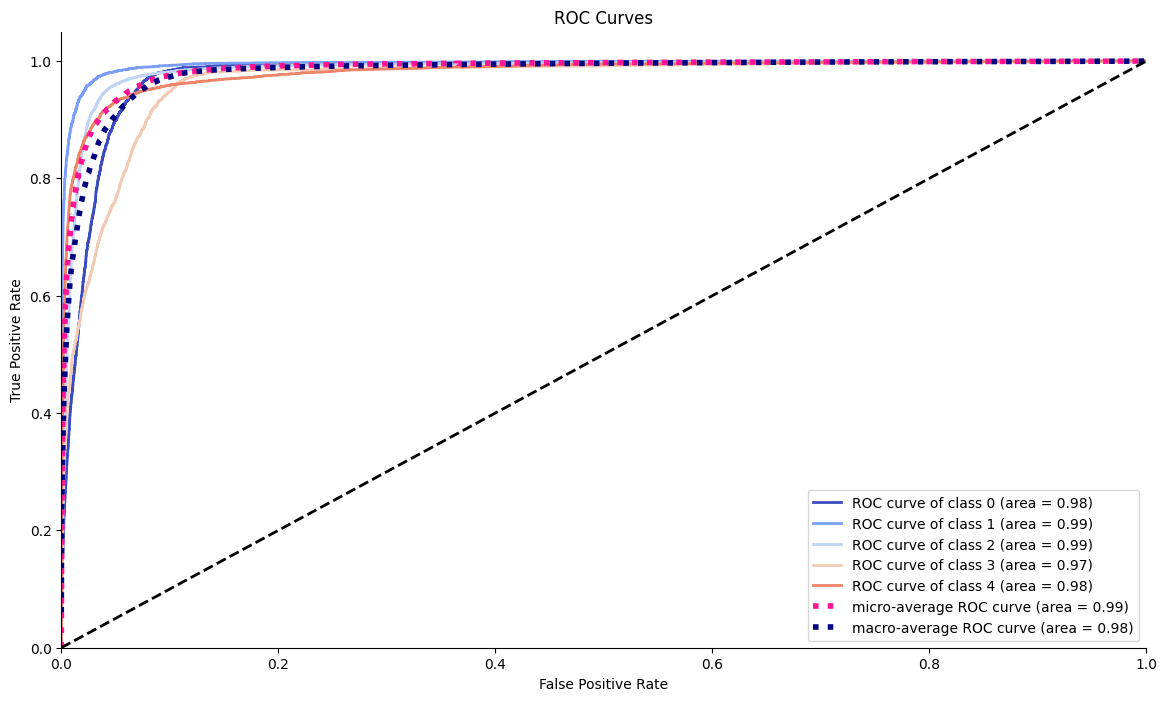
\includegraphics[width=9cm,height=6cm]{roc_auc_curve.png}
    \caption{ROC AUC Curve}
    \label{fig: sequence diagram}
\end{figure}

A ROC (Receiver Operating Characteristic) curve is a metric that shows how well a classifier system can diagnose problems as the discrimination threshold is changed. Plotting the true positive rate (TPR) at different categorization thresholds on the Y-axis and the false positive rate (FPR) on the X-axis results in the curve. A measure of how well a model can categorize data points is the area under the ROC curve (AUC), which can be computed.
\par
The model's achievement of a relatively high Area under the ROC curve (AUC score) is evident. This suggests that the model is a competent classifier because the model's predictions are of a high caliber.

We've seen that the model has a reasonable level of confidence in each and every prediction. We also observe a logical flow among the segmented sentences.

\begin{figure}
    \centering
    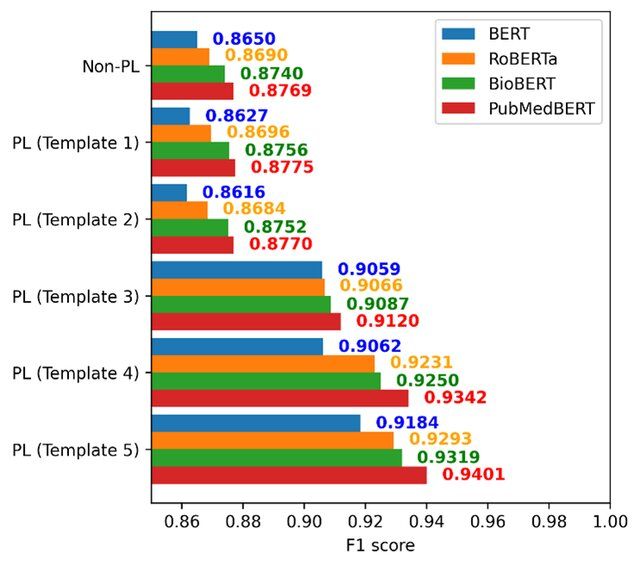
\includegraphics[width=9cm]{f1score.jpeg}
    \caption{f1 Score}
    \label{fig: sequence diagram}
\end{figure}





\newpage
\section{Conclusion and Future Scope}
The project exhibits promising avenues for future exploration and enhancement. To further improve upon the achieved accuracy of 88.4\% using Microsoft PubMedBERT, several avenues can be pursued. Firstly, refining hyperparameter tuning procedures, such as optimizing learning rates, batch sizes, and regularization techniques, could potentially boost model performance. Additionally, exploring alternative pre-processing techniques, such as data augmentation or advanced tokenization methods, may enhance the model's ability to capture subtle nuances in medical abstracts. Furthermore, incorporating ensemble learning approaches, where multiple models are combined to make predictions, could lead to improved classification accuracy and robustness. 
\par
We could explore the integration of multi-task learning techniques to enhance the model's capabilities.
By training PubMedBERT on multiple related tasks simultaneously, such as medical entity recognition, relation extraction, and document classification, the model can learn to extract richer representations of biomedical text and improve its understanding of complex relationships within medical documents. This approach not only expands the model's applicability but also fosters a deeper understanding of biomedical data, paving the way for more advanced biomedical applications such as clinical decision support systems, drug discovery, and personalized medicine.
\section*{Acknowledgment}

This work is being done as part of an undergraduate project at the IT department of PICT, PUNE.We appreciate all of the department's assistance with it.



\begin{thebibliography}{00}
\bibitem{b1} Franck Dernoncourt and Ji Young Lee, "PubMed 200k RCT: a Dataset for Sequential Sentence Classification in Medical Abstracts," 2017 In Proceedings of the Eighth International Joint Conference on Natural Language Processing (Volume 2: Short Papers), pages 308–313, Taipei, Taiwan. Asian Federation of Natural Language Processing.
\bibitem{b2} A. Brack, A. Hoppe, P. Buschermohle and R. Ewerth, "Cross-Domain Multi-Task Learning for Sequential Sentence Classification in Research Papers," in 2022 ACM/IEEE Joint Conference on Digital Libraries (JCDL), Cologne, Germany, 2022 pp. 1-13.
\bibitem{b3} Soumya Banerjee, Debarshi Kumar Sanyal, Samiran Chattopadhyay, Plaban Kumar Bhowmick, and Partha Pratim Das. 2020. Segmenting Scientific Abstracts into Discourse Categories: A Deep Learning-Based Approach for Sparse Labeled Data. In Proceedings of the ACM/IEEE Joint Conference on Digital Libraries in 2020 (JCDL '20). Association for Computing Machinery, New York, NY, USA, 429–432. https://doi.org/10.1145/3383583.3398598
\bibitem{b4} Di Jin and Peter Szolovits,"Hierarchical Neural Networks for Sequential Sentence Classification in Medical Scientific Abstracts," 2018 In Proceedings of the 2018 Conference on Empirical Methods in Natural Language Processing, pages 3100–3109, Brussels, Belgium. Association for Computational Linguistics.

\bibitem{b5} Xichen Shang, Qianli Ma, Zhenxi Lin, Jiangyue Yan, and Zipeng Chen, "A Span-based Dynamic Local Attention Model for Sequential Sentence Classification," 2021 In Proceedings of the 59th Annual Meeting of the Association for Computational Linguistics and the 11th International Joint Conference on Natural Language Processing (Volume 2: Short Papers), pages 198–203, Online. Association for Computational Linguistics.
\bibitem{b6} Hassanzadeh H, Groza T, Hunter J. Identifying scientific artefacts in biomedical literature: the Evidence Based Medicine use case. J Biomed Inform. 2014 Jun;49:159-70. doi: 10.1016/j.jbi.2014.02.006. Epub 2014 Feb 14. PMID: 24530879.
\bibitem{b7} Adam Gabriel Dobrakowski, Agnieszka Mykowiecka, Małgorzata Marciniak, Wojciech Jaworski, Przemysław Biecek, "Interpretable segmentation of medical free-text records based on word embeddings." in Journal of Intelligent Information Systems, 2021, 
https://doi.org/10.1007/s10844-021-00659-4.
\bibitem{b8} Yan Hu, Yong Chen, Hua Xu, "Towards More Generalizable and Accurate Sentence Classification in Medical Abstracts with Less Data" Springer (Journal of Healthcare Informatics Research), 2023. 
https://doi.org/10.1007/s41666-023-00141-6
\bibitem{b9} Arman Cohan, Iz Beltagy, Daniel King, Bhavana Dalvi, Daniel S. Weld. "Pretrained Language Models for Sequential Sentence Classification." Proceedings of the 2019 Conference on Empirical Methods in Natural Language Processing and the 9th International Joint Conference on Natural Language Processing (EMNLP-IJCNLP) (2019). https://doi.org/10.48550/arXiv.1909.04054
\bibitem{b10} Jeremy Howard, Sebastian Ruder, "Universal Language Model Fine-tuning for Text Classification.", Computation and Language (cs.CL); Machine Learning (cs.LG); Machine Learning (stat.ML), ACL 2018.
https://doi.org/10.48550/arXiv.1801.06146
\bibitem{b11} Xuelian Deng, Yuqing Li, Jian Weng and Jilian Zhang. "Feature selection for text classification: A review." Multimed Tools Appl 78, 3797–3816 (2019).
https://doi.org/10.1007/s11042-018-6083-5
\bibitem{b12} Jason Wei, Kai Zou. "EDA: Easy Data Augmentation Techniques for Boosting Performance on Text Classification Tasks" EMNLP-IJCNLP 2019 short paper. https://doi.org/10.48550/arXiv.1901.11196
\bibitem{b13} Shervin Minaee, Nal Kalchbrenner, Erik Cambria, Narjes Nikzad, Meysam Chenaghlu, Jianfeng Gao. "Deep Learning Based Text Classification: A Comprehensive Review" Computation and Language (cs.CL); Machine Learning (cs.LG); Machine Learning (stat.ML), 2021. 
https://doi.org/10.48550/arXiv.2004.03705
\end{thebibliography}
\vspace{12pt}

\end{document}
